\documentclass[a4paper,10pt]{article}

% Packages
\usepackage[utf8]{inputenc}
\usepackage[T1]{fontenc}
\usepackage[margin=1.5cm]{geometry}
\usepackage{paracol}
\usepackage{graphicx}
\usepackage{setspace}
\usepackage{enumitem}
\usepackage{titlesec}
\usepackage{tabularx}
\usepackage{tikz}
\usepackage[most]{tcolorbox}
\usepackage{fancyhdr}
\usepackage{longtable}
\usepackage[hidelinks]{hyperref} % legg til i preamble

% Fonts ---
\usepackage{fontspec}
\setmainfont{Roboto} % Change to your preferred font


\newfontfamily\ubuntu[
    Path = ../fonts/,
    UprightFont = Ubuntu-Regular.ttf,
    BoldFont    = Ubuntu-Bold.ttf,
    ItalicFont  = Ubuntu-Italic.ttf,
    BoldItalicFont = Ubuntu-BoldItalic.ttf
]{Ubuntu}
% Fonts ---

% Section title style (uppercase, spaced)
\titleformat{\section}{\bfseries\uppercase}{\thesection}{0.5em}{}

% No numbering
\setcounter{secnumdepth}{0}

% Reduce space between items
\setlist[itemize]{nosep,left=0pt}

% setup for header and footer
\pagestyle{fancy}
\fancyhf{} % Clear all header and footer fields

% Header
\fancyhead[L]{CV / \textbf{Elias Elfarri}}
\fancyhead[C]{+47 45 18 27 12 | moelfarri@gmail.com}
\fancyhead[R]{\textbf{Mobilutvikler}}
\fancyfoot[C]{\thepage}
\renewcommand{\headrulewidth}{0.5pt}
\setlength{\headheight}{12pt}
\setlength{\headsep}{40pt}

% FOOTER (line + centered page number)
\fancyfoot[C]{\thepage}
\renewcommand{\footrulewidth}{0.5pt}
\setlength{\footskip}{20pt}     % distance from text to footer
 


\begin{document}
% --- Side 1 starter her fra ---

% Space before content
\vspace{3em}

\begin{paracol}{2}
% ----- Left column -----
\begin{flushleft}
    % Profile picture
    \begin{tikzpicture}
     \clip (0,1.5) circle (2cm); % adjust size (radius)
     \node at (0,0) {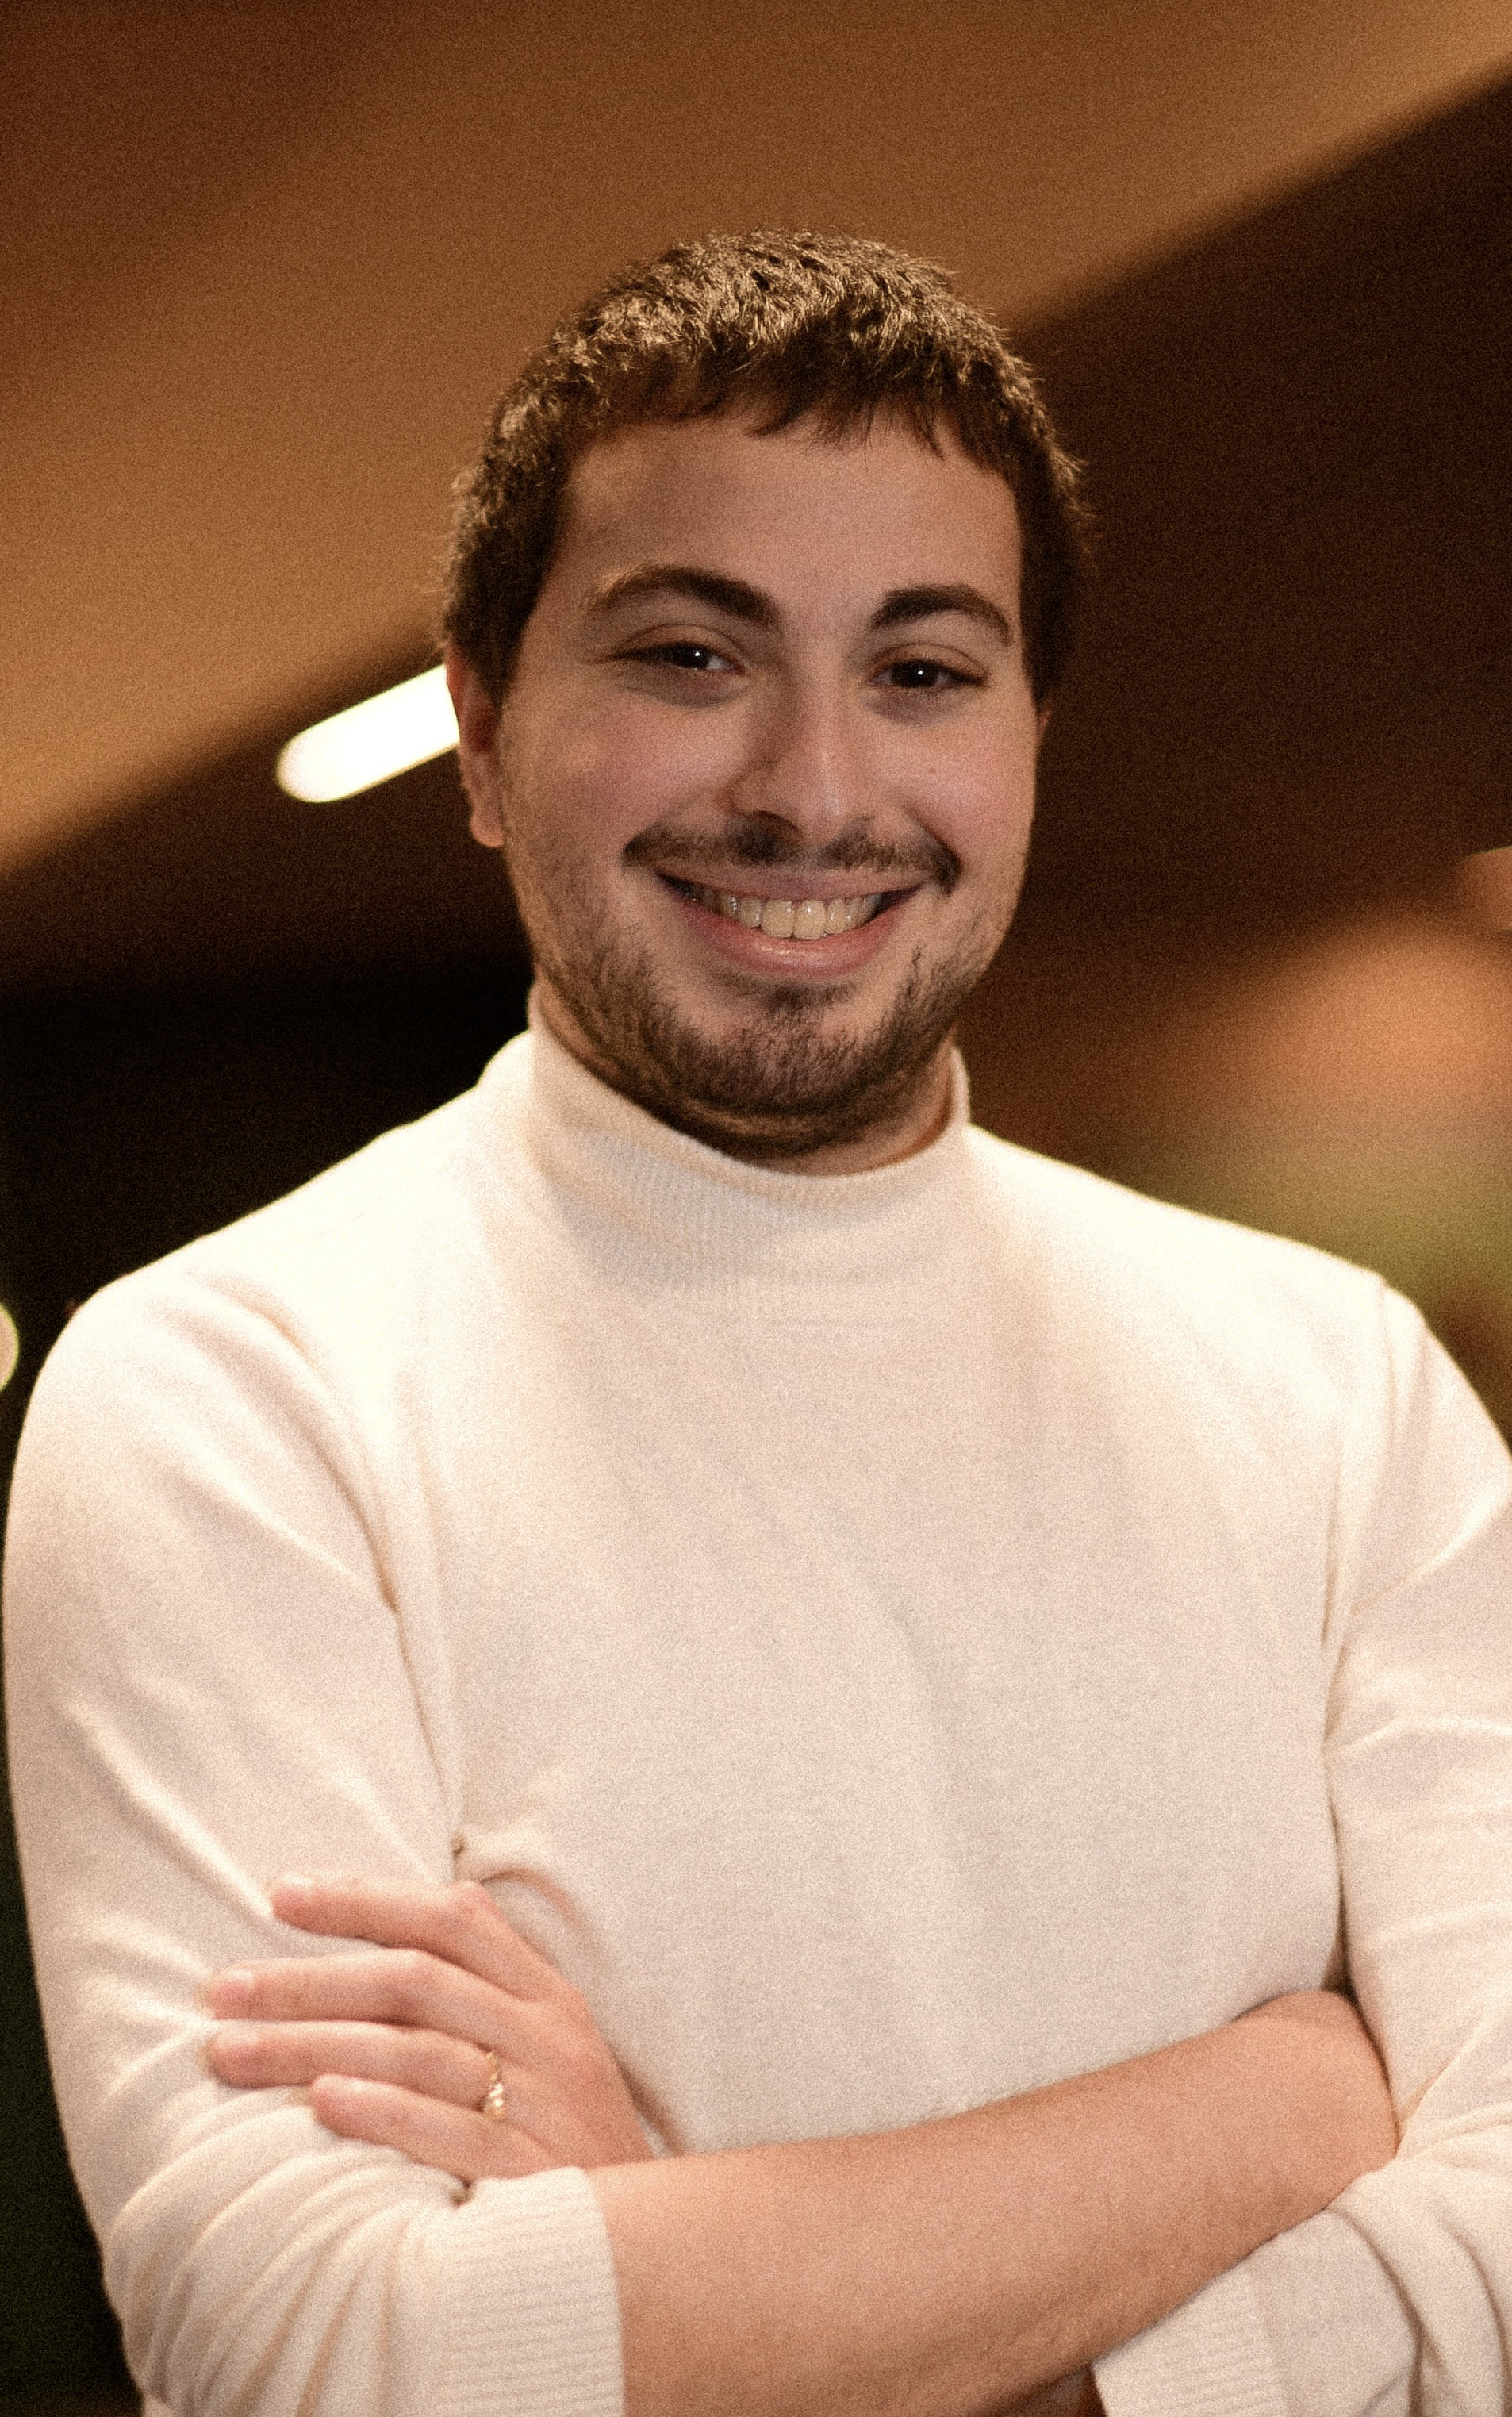
\includegraphics[width=5cm]{../portrait.jpg}};
    \end{tikzpicture}

    % a bar between image and name
    \vspace{1em}
    \noindent\rule{4cm}{10pt}
    

    \vspace{1.5em}
    {\Huge \ubuntu{Elias Elfarri}} \\
    \vspace{0.5em}
    
    \begin{tcolorbox}[
        colback=white,       % background color
        colframe=white,      % border color
        boxrule=0.0pt,       % border thickness
        arc=2mm,             % rounded corners
        width=0.85\linewidth,% make box narrower than column
        left=0mm, right=2mm, top=1mm, bottom=1mm % inner padding
        ]
    
    Elias er en mobilutvikler med 
    fire års erfaring fra både native-utvikling
     i Swift og Kotlin og kryssplattform med Flutter/Dart.
      Han har bygget opp mobilteam,
       ledet utviklingen av skalerbare
        kodebaser og publisert syv apper 
        på App Store og Google Play. 
        Med erfaring som spenner fra BLE,
         kamera og sanntids grafer til widgets 
         og spesialisert hardware-integrasjon,
          behersker han hele spekteret av
           mobilutvikling.
      Han er kjent som initiativrik, 
      reflektert og har gode pedagogiske evner.
       Elias leder Flutter Meetup-nettverket i 
       Oslo/Norge med over 500 medlemmer,
        hvor han arrangerer samlinger, 
        kurs og hackathons. 
        Dette engasjementet 
        gjør ham til en pådriver som både løfter
         prosjekter og kolleger.
    \end{tcolorbox}
\end{flushleft}

\switchcolumn

\vspace{5em}
\begin{center}
    
\end{center}
\vspace{2em}

% ----- Right column -----
 
\section{\ubuntu ERFARING}
\renewcommand{\arraystretch}{1.3} % Spacing between rows
\begin{tabularx}{\columnwidth}{@{}lX@{}}
2022 -- d.d & Fink AS, Mobilutvikler \\
2023 -- 2025 & Fink AS, Fagansvarlig Mobilutvikling \\
2021 -- 2022 & DNV, Frontend utvikler \\
2019 -- 2020 & Jenteprosjektet Ada, Prosjekt assistent \\
2018 -- 2022 & SIT, Team leder \\
2017 -- 2018 & NVFT AS, Promotør \\
2015 -- 2016 & Oslo Kommune, Hjelpepleier \\
\end{tabularx}

% space and line
\vspace{0.5em} 
\noindent\rule{\linewidth}{0.2pt}

\section{\ubuntu Utdanning}
\renewcommand{\arraystretch}{1.3} % Spacing between rows
\begin{tabularx}{\columnwidth}{@{}l>{\raggedright\arraybackslash}X@{}}
2017 -- 2022 & Norges teknisk-naturvitenskapelige universitet, Master i kybernetikk og robotikk, Sivilingeniør \\
2017 -- 2017 & Université de Caen Normandie, Utveksling \\
2016 -- 2017 & Norges teknisk-naturvitenskapelige universitet, Årsstudium i Fransk språk og litteratur \\
\end{tabularx}

% space and line
\vspace{0.5em} 
\noindent\rule{\linewidth}{0.2pt}


\section{\ubuntu Kunder}
DNV, \hspace{0.1em} 
InlineX, \hspace{0.1em} 
Norges teknisk-naturvitenskapelige
universitet

% space and line
\vspace{0.5em} 
\noindent\rule{\linewidth}{0.2pt}

\section{\ubuntu Roller}
Tech lead, \hspace{0.1em}
Mobilutvikler, \hspace{0.1em}
Frontend utvikler, \hspace{0.1em}
Fagansvarlig

\end{paracol}

\newpage
% --- Side 2 starter her fra ---

 % --- Verv seksjon ---
\section{Verv}
\begin{tabularx}{\linewidth}{@{}lX@{}}
2023 -- d.d & Flutter Oslo Meetup gruppe, Arrangør og leder \\
2024 -- d.d & Flutter and Friends Conference Stockholm, Arrangør \\
2018 -- 2019 & ISFiT, Dialog koordinator \\
\end{tabularx}
\vspace{1em}

 % --- Publikasjoner seksjon ---
\section{Publikasjoner}
\begin{tabularx}{\linewidth}{@{}lX@{}}
Sep.2025 & 
Konferanseforedrag, Either This or That: Expressive Error-Handling in Dart \\
Jan.2025 & 
\href{https://www.kode24.no/artikkel/derfor-bor-du-velge-flutter-i-2025/82529763}{kode24 artikkel, Derfor bør du velge Flutter i 2025!} \\
Nov.2024 & 
\href{https://www.kode24.no/artikkel/mener-det-er-tull-at-det-ikke-satses-pa-flutter-men-dart-er-en-flaskehals/82169214}{kode24 artikkel, Mener det er tull at det ikke satses på Flutter: – Men Dart er en flaskehals} \\
Apr.2023 & 
\href{https://ieeexplore.ieee.org/document/10093855/citations?tabFilter=papers\#citations}{Publikasjon av masteroppgaven, Artificial Intelligence-Driven Digital Twin of a Modern House Demonstrated in Virtual Reality} \\
\end{tabularx}
\vspace{1em}

% --- Stor tittel for prosjekter ---
\section{{\Huge \ubuntu PROSJEKTER}}


% --- Erfaring ---
\noindent
\begin{longtable}{@{}p{4cm}p{11cm}@{}}  % venstre = bredere, høyre = beskrivelse
\textbf{InlineX}
& \textbf{Prosjekt:} tekst kommer \\
Produksjonsfasen & \\
Jan.2026 - Jun.2026 & \\
& \\
&  \textbf{Rolle:} \\
& \\
& \textbf{Kompetanser:} \\
\end{longtable}

\vspace{2em}



% --- Erfaring ---
\noindent
\begin{longtable}{@{}p{4cm}p{11cm}@{}}  
\textbf{InlineX} 
& \textbf{Prosjekt:} I 2025 gikk InlineX inn i produksjonsfasen av Stream-prosjektet. Selskapet har blitt en scale-up og  har vokst til å være 21 \\
Produksjonsfasen &  ansatte. Målet med prosjektet var å videreutvikle selskapets native prosjekter for iOS og Android, redusere kostnader ved å erstatte \\
Jan.2025 -- Des.2025 &  dedikerte hardware-enheter med mobilapper og BLE-baserte IoT-løsninger, samt gjøre distribusjon og vedlikehold mer effektivt. InlineX Stream ble bygget for å digitalisere testing av sikkerhetsventiler (0–400 bar) i energi- og offshore-sektoren, og innen Q4 2025 ble løsningen lansert til betalende kunder. Som Tech Lead for mobil hadde Elias det overordnede ansvaret for monorepo-arkitekturen, programvarekvalitet og tekniske beslutninger. Prosjektet inkluderte videreutvikling av mobil monorepoen med tre apper, 20+ interne pakker, tre first-party plugins, og et stadig mer modent in-house designsystem. \\
& \\
& Elias etablerte en vertical slices og  micro-frontends arkitektur for å gjøre det enkelst mulig for nye utviklere å komme i gang og bidra i den etterhvert voksende native infrastrukturen. Dette gjorde at utviklere på teamet kunne jobbe på spesifikke features isolert fra alle andre kontekster, og dermed øke produktiviteten. Han sikret arkitekturens robusthet gjennom 400+ custom lint-regler, codegen-verktøy og dokumentasjon. Dette sikret at teamet kunne komfortabelt skrive kode de var trygge på, enten med Flutter/Dart, rent Native med Kotlin/Swift eller annen relevant teknologi. Teamet var blitt et Native Platforms team. \\
& \\
& I tillegg så fikk Elias på plass en del agentisk AI infrastruktur (relevant MCP-kontekst, MD-dokumentasjon, subagenter, etc) som gjorde det enkelt å tilrettelegge for utviklerne og bruke verktøyet de likte best (Claude Code, GitHub Copilot, Gemini m.fl.).  \\
& \\
& Han fikk også på plass SwiftUI-baserte grafer, en egen AVFoundation/CameraX-plugin for kamera, og videre modning av CoreBluetooth- og Android BLE-koden for stabilitet i produksjon. Som leder for mobilteamet hadde Elias ansvar for onboarding, ressursplanlegging, stakeholder management og leveranser. Han bidro i over 20 tekniske intervjuer for mobil, embedded og cloud-roller, og bidro aktivt i selskapets oppskalering. Han satte opp en self-hosted CI/CD-agent (M4 Mac Mini) for signering og distribusjon til TestFlight og Google Play, samt for å kjøre tunge E2E-tester (Maestro) som ikke kunne håndteres på Microsofts hosted agenter. Han samarbeidet med jurister om privacy policy og GDPR compliance, flyttet appene fra privat appstore til offisielle appstores for å redusere kostnader, og sikret samtidig at InlineX Stream og de andre applikasjonene kunne drives og videreutvikles trygt i en produksjonssetting. \\
& \textbf{Rolle:} Tech Lead, mobilutvikler, prosjektleder. \\
& \\
& \textbf{Kompetanser:} Flutter, Dart, Kotlin, Swift, SwiftUI, iOS, Android, CoreBluetooth, Android Bluetooth, ESP32, AVFoundation, CameraX, Objective-C, Java, C, IoT-integrasjon, mobil monorepo-arkitektur, vertical slices, micro-frontends, in-house design system, 400+ custom lint-regler, codegen-verktøy, RxDart, Bluetooth Low Energy, Widgetbook, flutter\_blue\_plus, Pub workspaces, Melos, Mason, UIKit, Android Settings Intents, DCM, Pigeon, Shorebird, Drift ORM/SQLite, Freezed, Build Runner, Golden testing, Unit Tests, Integration Tests, VSCode, Xcode, Android Studio, CI/CD (Azure DevOps, Fastlane, Maestro, xcodebuild, Fastlane Match, Fastlane Screenshot Automation, Fastlane Beta Deployment), self-hosted Mac Mini agent, TestFlight, Google Play Console, App Store Connect API, Firebase Crashlytics, Firebase Analytics, Firebase Performance Monitoring, Microsoft Clarity, Privacy Manifest, Privacy Policy, GDPR compliance, Google Cloud Console, stakeholder management, teamledelse, onboarding, rekruttering, backlog refinement, delivery management, produktstrategi, continuous discovery \& delivery, trio-modellen, Claude Code, Gemini, Copilot, Claude Desktop, ChatGPT Desktop. \\
\end{longtable}

\vspace{2em}

% --- Erfaring ---
\noindent
\begin{longtable}{@{}p{4cm}p{11cm}@{}}  % venstre = bredere, høyre = beskrivelse
\textbf{InlineX}
& \textbf{Prosjekt:} I 2024 ledet Elias oppstarten av InlineX Stream, selskapets hittil største mobilprosjekt, samtidig som han hadde ansvar for drift \\
Modningsfasen & av Insitu Sync. Stream-prosjektet kombinerte mobilutvikling med IoT og hardware-integrasjon, og hadde som formål å erstatte tidligere \\
Jan.2024 - Des.2024 & industrielle enheter til en verdi av rundt 2 millioner NOK med en løsning basert på app + Bluetooth-krets (ESP32). Resultatet var en reduksjon i produksjonskostnader til 150 000 NOK per enhet, lavere vedlikeholdskostnader og enklere hardware stack. På dette tidspunktet består teamet av en stadig voksende produktavdeling med folk på embedded, cloud, mobil, design og prosjektledelse. På teknisk side bygges den nye "Stream" appen av et inhouse design komponent bibliotek, first party native plugins og mange andre pakker takket være en monorepo arkitektur. Den viktigste featuren blir en tredelt BLE-løsning (native plugins i Swift/Kotlin, businesslogikk med egen GATT-protokoll, og UI/UX-lag).\\
& \\
&  \textbf{Rolle:} Som App Tech Lead hadde Elias overordnet ansvar for tre apper, teknisk retning for mobilavdelingen og ledelse av en annen juniorutvikler. Han drev rekruttering, opplæring, tekniske beslutninger og fungerte som bindeledd mellom produkt, design og ledelse. Han fasiliterte retroer, jobbet med OKRs, kvartalsvis estimater, stakeholder management og leveranser, samt bidro til selskapets produktstrategi og navnearbeid. I samarbeid med ledelsen bidro han til å transformere selskapet videre til et continuous discovery-produkt scale-up, hvor man organiserte arbeidet i trioer (produkteier, designer, tech lead) og bidro i å etablere et Domain Driven Design-rammeverk for felles begrepsbruk på tvers av organisasjonen. \\
& \\
& \textbf{Kompetanser:} Flutter, Dart, Kotlin, Swift, SwiftUI, Jetpack Compose, Objective-C, Android, iOS, Linux, ESP32, CoreBluetooth, Android Bluetooth API, BLE-arkitektur, gRPC, WebSockets, SQLite, Drift ORM, RxDart, Freezed, BLoC, Melos, Mason, Widgetbook, Azure DevOps, CI/CD, Figma, Figjam, Slack, stakeholder management, delivery management, OKRs, continuous discovery, trio-modellen, domain driven design modellering, teamledelse, rekruttering og produktstrategi.\\
\end{longtable}



\vspace{2em}

\noindent
\begin{longtable}{@{}p{4cm}p{11cm}@{}}  % venstre = bredere, høyre = beskrivelse
\textbf{InlineX}
& \textbf{Prosjekt:} I 2023 fortsatte Elias arbeidet med InlineX Mobile og tok  initiativ til å restrukturere kodebasen til et monorepo for å støtte \\
Restruktureringsfasen & utviklingen av flere enterprise nivå applikasjoner. Han utviklet blant annet Insitu Sync,  en applikasjon med robust online/offline-synkronisering,\\
Jan.2023 - Des.2023 & og bygde opp et enkelt designsystem i Figma inspirert av Material 3 og Atomic Design for gjenbruk av komponenter på tvers av web og mobil. Dette la grunnlaget for at teamet kunne levere nye produkter raskere og med høyere kvalitet. Samtidig tok Elias en nøkkelrolle i selskapets organisatoriske transformasjon. Han fikk ledelsen med på å hente inn nye roller – en ekstra utvikler, en designer og en prosjektleder (på kortere oppdrag) – noe som gjorde det mulig å etablere en mer moden produktutviklingskultur. Prosjektet markerte et vendepunkt der InlineX beveget seg fra prosjektorienterte fossefallsleveranser til å bygge en produktavdeling basert på agile prosesser, kontinuerlig discovery og tverrfaglig samarbeid.\\
& \\
& \textbf{Rolle:} Elias var både utvikler, arkitekt og endringsagent. Han tok initiativ til å etablere moderne arbeidsprosesser, fasiliterte retrospektiver og bidro aktivt til at selskapet innførte standups, sprintarbeid, OKRs, continuous discovery-trioer og stakeholder management. Han tok ansvar for å koble utvikling tettere på produkt- og forretningssiden, og sørget for at teamet hadde verktøyene og prosessene som trengtes for å skalere. \\
& \\
& \textbf{Kompetanser:} Flutter, Dart, Kotlin, Swift, Melos (monorepo), Widgetbook, Mason, Drift ORM/SQLite, RxDart, Freezed, Build Runner, Firebase Crashlytics, Azure DevOps (Git, Pipelines), VS Code, Android Studio, Xcode, Figma (Material 3, Atomic Design), Slack, Confluence, Jira, Monday, WebSockets, gRPC, stakeholder management, delivery management, OKRs, continuous discovery, fasilitering av retrospektiver, innføring av agile prosesser, produktstrategi og endringsledelse. \\
\end{longtable}


\vspace{2em}


% --- Erfaring ---
\noindent
\begin{longtable}{@{}p{4cm}p{11cm}@{}}  % venstre = bredere, høyre = beskrivelse
\textbf{InlineX}
& \textbf{Prosjekt:} Elias ble hentet inn som konsulent for å utvikle en kryssplattform applikasjon for iOS, Android og Linux, til bruk innen  energi- og\\
Startupfasen & offshore-sektoren. Oppdraget startet som en hasteløsning for kunder uten internett, men utviklet seg til å bli et strategisk produkt for \\
Aug.2022 - Des.2022 & selskapet. Elias besluttet å ta i bruk Flutter, og leverte allerede første måned en proof of concept, "InlineX Mobile", som fortsatt brukes i produksjon i dag. Løsningen ble tatt i bruk på installasjoner i blant annet Australia, Malaysia, Saudi-Arabia, Equinor Kollsnes, Nyhavna og Angola. Prosjektet markerte en av de første gangene Flutter antageligvis ble benyttet i oljebransjen.\\
& \\
& \textbf{Rolle:} Da Elias startet, bestod selskapet av kun åtte ansatte – uten etablert produktutviklingskultur, uten designer, og med kun to utviklere totalt, inklusiv Elias. Han ble derfor ikke bare mobilutvikler, men også arkitekt, strateg og pedagog. Elias hadde en sentral rolle i å forme både teknologivalg, utviklingspraksis og produktstrategi, og han konsulterte ledelsen i hvordan selskapet burde bevege seg fra ren bestillingsbasert utvikling til et moderne produkthus med egen produktavdeling. Han etablerte infrastruktur, innførte smidige utviklingsmetoder, og bygde opp grunnlaget for et bærekraftig produktmiljø. Over tid gikk han fra konsulent til å bli en nøkkelperson i selskapets teknologisatsning, med ansvar for leveranser og veiledning av andre utviklere. \\
& \\
& \textbf{Kompetanser:} Flutter, Dart, Kotlin, Swift, Android, iOS, Linux, Figma, Azure DevOps (Git, Pipelines), Firebase Crashlytics, SQLite, Riverpod, BLoC pattern, WebSockets, REST, RxDart, gRPC, KeyChain, MDM, Material Design 3, Widgetbook, Melos, Mason, Drift ORM, Shorebird, Pigeon, FFIgen, SwiftUI, Live Activities, Dynamic Island, TestFlight, Google Play Console, C++, BLE, Docker, Kubernetes, Maestro (integrasjonstesting), CI/CD, moderne produktutvikling og arkitektur. \\

\end{longtable}


\vspace{2em}

% --- Erfaring ---
\noindent
\begin{longtable}{@{}p{4cm}p{11cm}@{}}  % venstre = bredere, høyre = beskrivelse
\textbf{DNV} 
& \textbf{Prosjekt:} Elias har utviklet nye funksjoner i DP-CAP og DYN-CAP applikasjonene, brukt til beregninger og sertifisering av dynamisk pos-\\
Maritime Cybernetics Advisory & isjonering av skip. Han utviklet i Python/OpenCV basert på Watershed-metoden, som reduserte manuelt arbeid fra flere dager til sekunder, og som ble kritisk for sertifiseringsanalyser bestilt av kunder\\
2021 -- 2022 & som Equinor. Dette økte lønnsomheten av disse rapportene massivt, med en fastpris på 100 000 NOK så tok det et par klikk å levere samme analyse som kunne ta opp til en uke før. \\
& \\
& \textbf{Rolle:} Systemutvikler, backend, frontend, bildebehandlingsingeniør. \\
& \\
& \textbf{Kompetanser:} TypeScript, React, ClojureScript, Reframe, Clojure, Java, Python (OpenCV), Leiningen, Jenkins, bildebehandling/Computer Vision, PID-regulator, Watershed algoritmen og klassisk bildebehandling, dynamisk posisjonering, sertifisering av DP-systemer, maritim domeneforståelse, General Arrangement tegninger. \\
\end{longtable}


\vspace{2em}

% --- Erfaring ---
\noindent
\begin{longtable}{@{}p{4cm}p{11cm}@{}}  % venstre = bredere, høyre = beskrivelse
\textbf{NTNU} 
& \textbf{Prosjekt:} I masteroppgaven utviklet Elias en komplett digital tvilling av en bygning, kombinert med sensorteknologi, kunstig intelligens og \\
2021 -- 2022  & virtuell virkelighet. Prosjektet demonstrerte flere modenhetsnivåer av digitale tvillinger – fra standalone, beskrivende og diagnostiske modeller, til prediktive og preskriptive modeller. Løsningen inkluderte blant annet 3D-modellering (Revit/3DS Max), Unity-integrasjon med sanntidsdata fra IoT-sensorer, maskinlæringsbaserte prediksjonsmodeller, samt VR-grensesnitt for interaktive demonstrasjoner. Oppgaven ble belønnet med Tekna-stipend, omtalt i Teknas magasin, og videre publisert som vitenskapelig artikkel i IEEE. \\
& \\
& \textbf{Kompetanser:} Digital Twin, Kunstig intelligens (ML, RNN, LSTM, ensemblemetoder), IoT \& sensorteknologi, Virtuell virkelighet (Unity, Oculus Quest 2), 3D-modellering (Revit, 3DS Max), Python, C\#, Datadrevet modellering, Prediksjon og simulering, Xgboost/Catboost/LightGBM, Tensorflow/Keras, Pandas, Numpy, Matplotlib, TwinMotion, Blender, SolidWorks, Unreal Engine 4, Anaconda, Jupyter Notebook, Scikit, CUDA, ARIMA, LSTM, JavaScript, Express.js, Node.js, Philips Hue, Netatmo Weather Station, Disruptive Technlogies Sensorer. \\
\end{longtable}
 


 
\end{document}